%%%%%%%%%%%%%%%%%%%%%%%%%%%%%%%%%%%%%%%
% Wenneker Resume/CV
% LaTeX Template
% Version 1.1 (19/6/2016)
%
% This template has been downloaded from:
% http://www.LaTeXTemplates.com
%
% Original author:
% Frits Wenneker (http://www.howtotex.com) with extensive modifications by 
% Vel (vel@LaTeXTemplates.com)
%
% License:
% CC BY-NC-SA 3.0 (http://creativecommons.org/licenses/by-nc-sa/3.0/
%
%%%%%%%%%%%%%%%%%%%%%%%%%%%%%%%%%%%%%%

%----------------------------------------------------------------------------------------
%	PACKAGES AND OTHER DOCUMENT CONFIGURATIONS
%----------------------------------------------------------------------------------------

\documentclass[a4paper,12]{memoir} % Font and paper size

%%%%%%%%%%%%%%%%%%%%%%%%%%%%%%%%%%%%%%%%%
% Wenneker Resume/CV
% Structure Specification File
% Version 1.1 (19/6/2016)
%
% This file has been downloaded from:
% http://www.LaTeXTemplates.com
%
% Original author:
% Frits Wenneker (http://www.howtotex.com) with extensive modifications by 
% Vel (vel@latextemplates.com)
%
% License:
% CC BY-NC-SA 3.0 (http://creativecommons.org/licenses/by-nc-sa/3.0/)
%
%%%%%%%%%%%%%%%%%%%%%%%%%%%%%%%%%%%%%%%%%

%----------------------------------------------------------------------------------------
%	PACKAGES AND OTHER DOCUMENT CONFIGURATIONS
%----------------------------------------------------------------------------------------

\usepackage{XCharter} % Use the Bitstream Charter font
\usepackage[utf8]{inputenc} % Required for inputting international characters
\usepackage[T1]{fontenc} % Output font encoding for international characters

\usepackage[top=1cm,left=1cm,right=1cm,bottom=1cm]{geometry} % Modify margins

\usepackage{graphicx} % Required for figures

\usepackage{flowfram} % Required for the multi-column layout

\usepackage{url} % URLs

\usepackage[usenames,dvipsnames]{xcolor} % Required for custom colours

\usepackage{tikz} % Required for the horizontal rule

\usepackage{enumitem} % Required for modifying lists
\setlist{noitemsep,nolistsep} % Remove spacing within and around lists

\setlength{\columnsep}{\baselineskip} % Set the spacing between columns

% Define the left frame (sidebar)
\newflowframe{0.2\textwidth}{\textheight}{0pt}{0pt}[right]
\newlength{\LeftMainSep}
\setlength{\LeftMainSep}{0.2\textwidth}
\addtolength{\LeftMainSep}{1\columnsep}
 
% Small static frame for the vertical line
\newstaticframe{1.5pt}{\textheight}{\LeftMainSep}{0pt}
 
% Content of the static frame with the vertical line
\begin{staticcontents}{1}
\hfill
\tikz{\draw[loosely dotted,color=black,line width=1.5pt,yshift=0](0,0) -- (0,\textheight);}
\hfill\mbox{}
\end{staticcontents}
 
% Define the right frame (main body)
\addtolength{\LeftMainSep}{1.5pt}
\addtolength{\LeftMainSep}{1\columnsep}
\newflowframe{0.7\textwidth}{\textheight}{\LeftMainSep}{0pt}[main01]

\pagestyle{empty} % Disable all page numbering

\setlength{\parindent}{0pt} % Stop paragraph indentation

%----------------------------------------------------------------------------------------
%	NEW COMMANDS
%----------------------------------------------------------------------------------------

\newcommand{\userinformation}[1]{\renewcommand{\userinformation}{#1}} % Define a new command for the CV user's information that goes into the left column

\newcommand{\cvheading}[1]{{\Huge\bfseries\color{black} #1} \par\vspace{.6\baselineskip}} % New command for the CV heading
\newcommand{\cvsubheading}[1]{{\Large\bfseries #1} \bigbreak} % New command for the CV subheading

\newcommand{\Sep}{\vspace{1em}} % New command for the spacing between headings
\newcommand{\SmallSep}{\vspace{0.5em}} % New command for the spacing within headings

\newcommand{\aboutme}[2]{ % New command for the about me section
\textbf{\color{black} #1}~~#2\par\Sep
}
	
\newcommand{\CVSection}[1]{ % New command for the headings within sections
{\Large\textbf{#1}}\par
\SmallSep % Used for spacing
}

\newcommand{\CVItem}[2]{ % New command for the item descriptions
\textbf{\color{Black} #1}\par
#2
\SmallSep % Used for spacing
}

\newcommand{\bluebullet}{\textcolor{Black}{$\circ$}~~} % New command for the blue bullets
 % Include the file specifying document layout and packages

\usepackage{hyperref,xcolor}

%----------------------------------------------------------------------------------------
%	NAME AND CONTACT INFORMATION 
%----------------------------------------------------------------------------------------

\userinformation{ % Set the content that goes into the sidebar of each page
\begin{flushright}
% Comment out this figure block if you don't want a photo
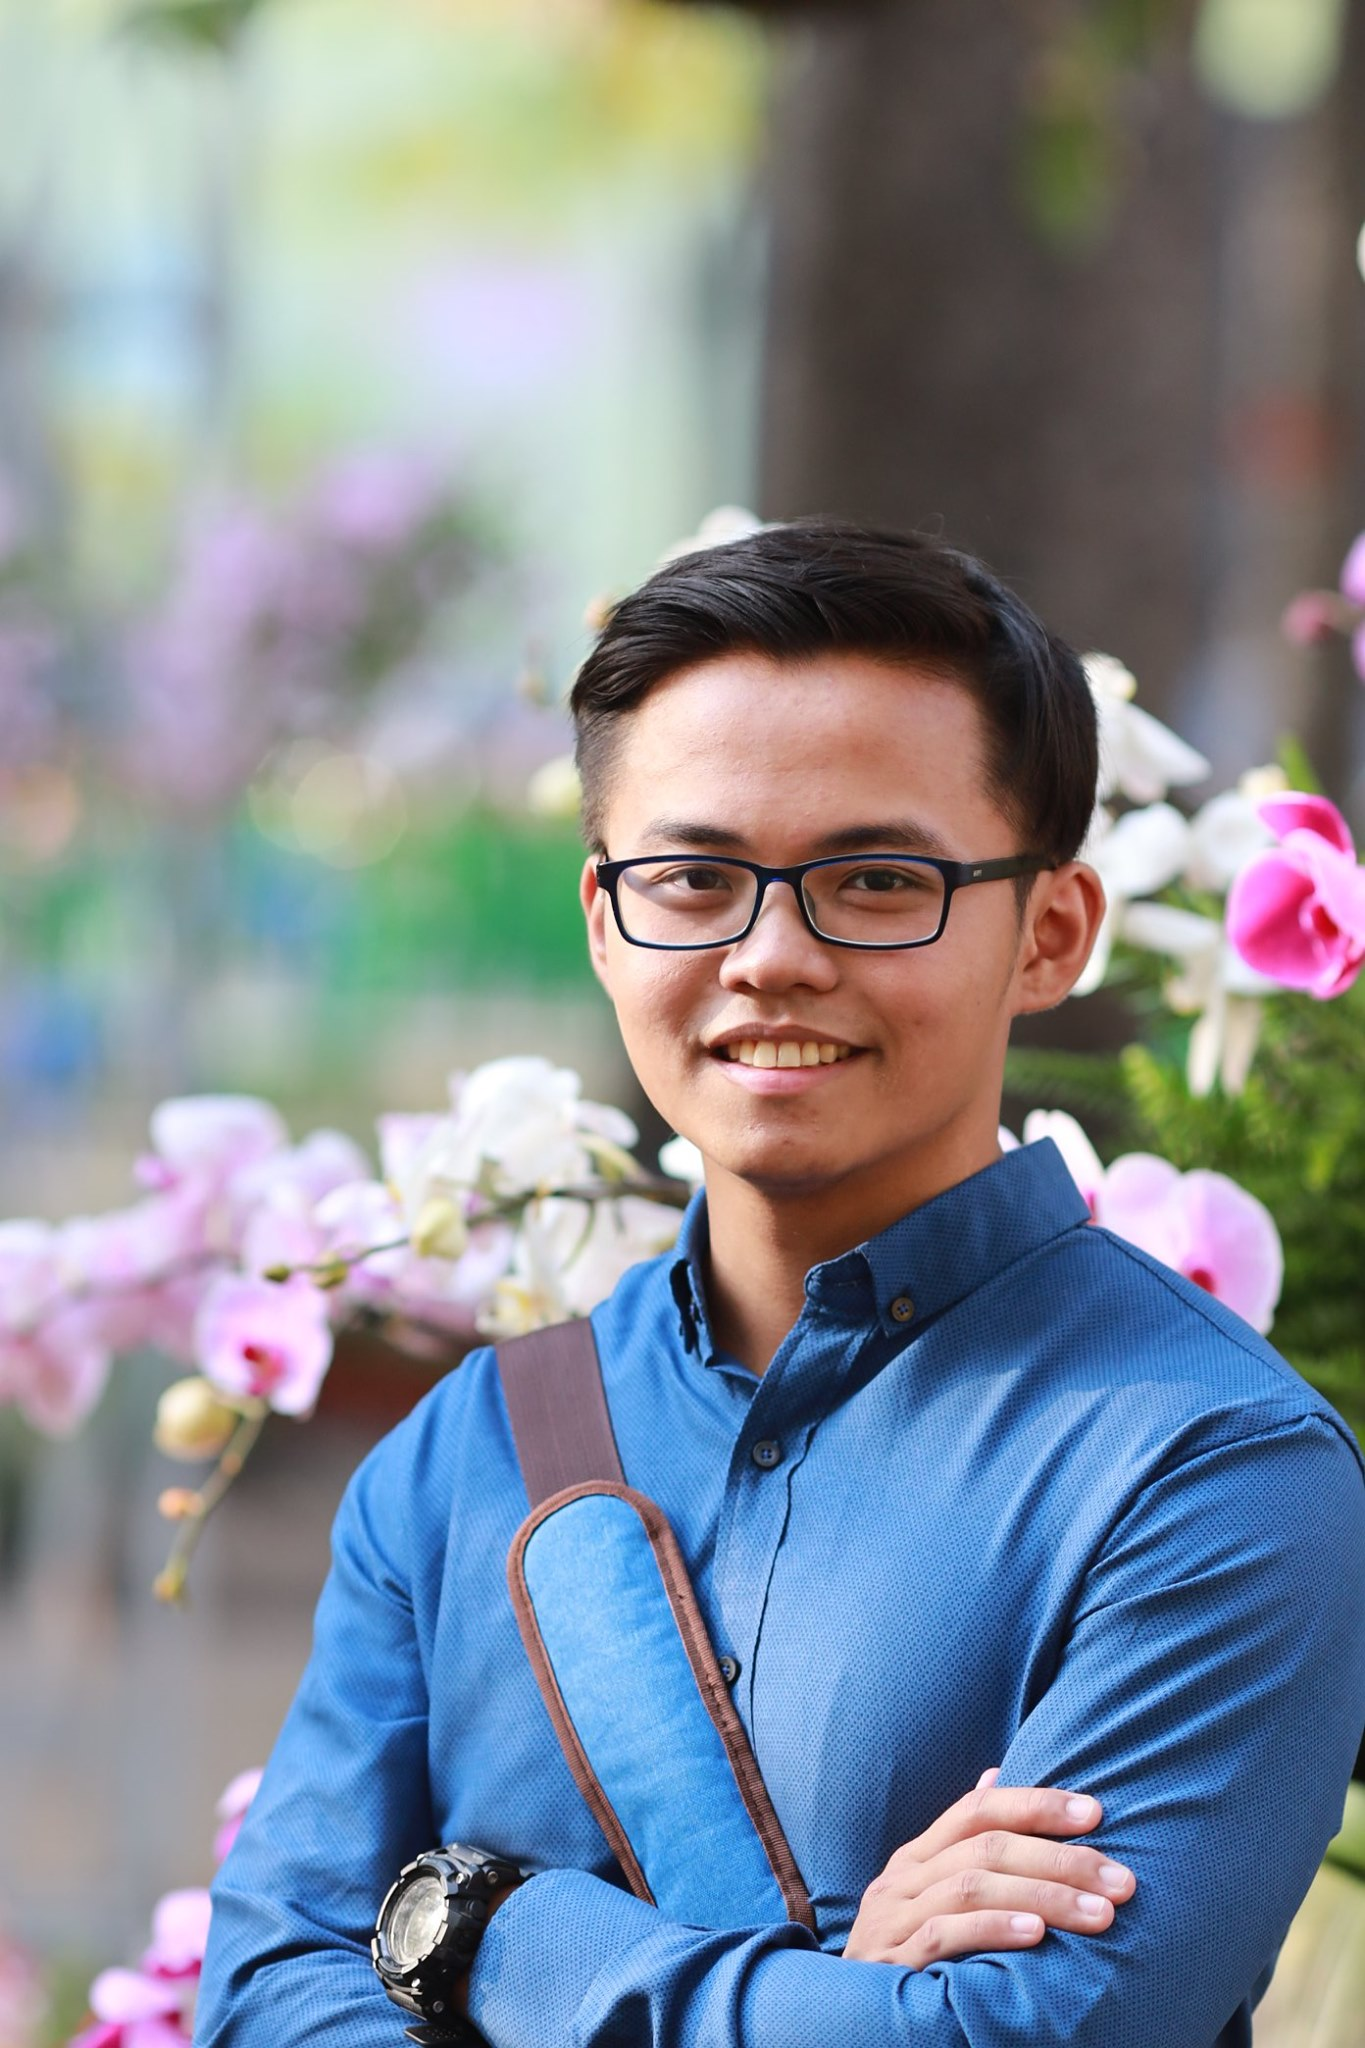
\includegraphics[width=1\columnwidth]{LinkedInAva2020.jpg}\\[\baselineskip] % Your photo
\small % Smaller font size
Ted Vu \\ % Your name
\url{tedvu184@gmail.com} \\ % Your email address
\href{tedvu.netlify.app//}{Personal Blog} \\ % Your URL
(04) 2699 1804 \\ % Your phone number
\Sep % Some whitespace
\textbf{Address} \\
85 Whitehall St \\ % Address 1
Footscray, Melbourne \\ % Address 2
Australia \\ % Address 3
\vfill % Whitespace under this block to push it up under the photo
\end{flushright}
}

%----------------------------------------------------------------------------------------

\begin{document}

\userinformation % Print your information in the left column

\framebreak % End of the first column

%----------------------------------------------------------------------------------------
%	HEADING
%----------------------------------------------------------------------------------------

\cvheading{Ted Vu} % Large heading - your name

\cvsubheading{Software Engineer} % Subheading - your occupation/specialization

%----------------------------------------------------------------------------------------
%	ABOUT ME
%----------------------------------------------------------------------------------------

\aboutme{About Me}{I'm currently an Analyst Programmer Intern at Momentum Systems and a third year undergrad Software Engineering student at RMIT University. I have a strong interest in building things and figuring out how things work whether it is physical objects or an Algorithms, this is the main reason I decided to pursuit a career in Software Engineering. My number one priority right now is to learn as much as I can from my talented and knowledgeable coworker at Momentum Systems. }

%----------------------------------------------------------------------------------------
%	EDUCATION
%----------------------------------------------------------------------------------------

\CVSection{Education}

%------------------------------------------------

\CVItem{2018 - 2021, RMIT University - GPA: 3.9/4.0}{Bachelor of Software Engineering}


%------------------------------------------------
\CVItem{2017 - 2018, RMIT University Vietnam - GPA: 4.0/4.0}{Bachelor of Engineering (Software Engineering)(Honours)}

\Sep % Extra whitespace after the end of a major section

%----------------------------------------------------------------------------------------
%	EXPERIENCE
%----------------------------------------------------------------------------------------

\CVSection{Experience}

%------------------------------------------------

\CVItem{August 2020 - present, \textit{Analyst Programmer Intern}}{}
\CVItem{Momentum Systems, Melbourne VIC}{}
\CVItem{\bluebullet{\textbf{Responsibility:}\textnormal{Develop features for core system, customize software according to user requirements and support customers on demand.}}}

\Sep % Extra whitespace after the end of a major section

\CVItem{November 2018 - Jan 2019, \textit{Casual Waiter Staff}}{}
\CVItem{ Chu The Pho, Melbourne VIC}{}
\CVItem{\bluebullet{\textbf{Responsibility:} \textnormal{Serving food and taking order from customers.}}}

\Sep % Extra whitespace after the end of a major section

%----------------------------------------------------------------------------------------
%	ACHIEVEMENT
%----------------------------------------------------------------------------------------

\CVSection{Achievement}

%------------------------------------------------

\CVItem{August 2020, \textit{Winning first place ANZAC Regional Programming Contest}}{}
\CVItem{\bluebullet{\textbf{Result:} \textnormal{Collaborate with team members achieving the first place out of more than 30 teams across Pacific Region.}}}{}
 \bluebullet{\textbf{Certificate:} \href{https://www.dropbox.com/s/i4olkhqdw6hyni9/Certificate-Participation%20-%20ANZAC%204%20-%20Ted.pdf?dl=0}{Link}}

%------------------------------------------------
\Sep 

\CVItem{July 2017, \textit{Software Engineering Scholarship at RMIT University Vietnam}}\bluebullet{Recipient of Software Engineering Scholarship from RMIT University Vietnam for high achieving high school student}

%------------------------------------------------

\Sep % Extra whitespace after the end of a major section

%----------------------------------------------------------------------------------------
%	SKILLS
%----------------------------------------------------------------------------------------

\CVSection{Software Development Skills}

%------------------------------------------------

\CVItem{Programming}
{\begin{tabular}{p{0.2\textwidth} p{0.2\textwidth} p{0.2\textwidth}}
\bluebullet Java &  \bluebullet JavaScript & \bluebullet HTML/CSS\\
\bluebullet C++ &  \bluebullet PHP & \bluebullet SQL\\
\end{tabular}}

%------------------------------------------------
\Sep
\CVItem{Libraries and Frameworks}
{\begin{tabular}{p{0.2\textwidth} p{0.2\textwidth} p{0.2\textwidth}}
 \bluebullet React &  \bluebullet Spring & \bluebullet Boostrap\\
 \bluebullet GatsbyJS &  \bluebullet NodeJS\\
\end{tabular}}

%------------------------------------------------

\Sep
\CVItem{Software Development tools and technologies}
{\begin{tabular}{p{0.2\textwidth} p{0.2\textwidth} p{0.2\textwidth}}
 \bluebullet Git/Github &  \bluebullet Docker & \bluebullet CircleCI\\
 \bluebullet Unix/Linux &  \bluebullet NixOS\\
\end{tabular}}

%------------------------------------------------

\Sep % Extra whitespace after the end of a major section

%----------------------------------------------------------------------------------------
%	NEW PAGE DELIMITER
%	Place this block wherever you would like the content of your CV to go onto the next page
%----------------------------------------------------------------------------------------

\CVSection{Referee}

%------------------------------------------------

\CVItem{Dr.Fengling Han - Senior Lecturer in Computer Science Department RMIT University}{\textbf{Recommendation Letter:} \href{https://www.dropbox.com/s/0fmg4xnys9h7dlw/Ted_Letter.pdf?dl=0}{Letter} }


\clearpage % Start a new page

\userinformation % Print your information in the left column

\framebreak % End of the first column

%----------------------------------------------------------------------------------------
%   REFEREE
%----------------------------------------------------------------------------------------


%------------------------------------------------

\Sep % Extra whitespace after the end of a major section

%----------------------------------------------------------------------------------------
%	PROJECTS
%----------------------------------------------------------------------------------------

\CVSection{Extracurricular activity}

%------------------------------------------------

\CVItem{CSIT mentor}\bluebullet{Training Certificate: \href{https://www.dropbox.com/s/y1xjml3q9t92xvf/s3678491.pdf?dl=0}{Certificate} }

\Sep 

\CVItem{Enactus Non-profit organization member}\bluebullet{Task: Organize key events and come up with team member evaluation method }

\Sep

\CVSection{Key Projects}

%------------------------------------------------

\CVItem{May 2020, Demo Registration System}{\bluebullet{\textbf{Github:} \url{https://github.com/kevinvu184/SpreadsheetWebRegistration}}\\ \\ \bluebullet{\textbf{Responsibility:} Front end validation and design, implemented locking mechanism for concurrency control, designing database and helping with Back end development.} \\ \\ \bluebullet{\textbf{Project Description:} A side project developed under guidance of Network Programming course coordinator Dr. Fengling Han. The project had been used by RMIT Staff and around 130 students in the course to save the administration time.} \\ \\ \bluebullet{\textbf{Tools and Technologies:} Implemented in PHP, used Google Spreadsheet APIs, hosted on Apache Server.} }

\Sep 

\CVItem{December 2019, Lunardo Cinema Website}{\bluebullet{\textbf{Github:} \url{https://github.com/Ted-Vu/Lunardo-Cinema-Website}}\\ \\ \bluebullet{\textbf{Responsibility:} Front end design and development using pure HTML/CSS/JS and back end booking system with PHP.} \\ \\ \bluebullet{\textbf{Project Description:} An Assignment in Web Programming Course, High Distinction mark for this project (49.5/50) – Website being used as teaching material in future.} \\ \\ \bluebullet{\textbf{Tools and Technologies:} The website was created by leveraging knowledge in HTML/CSS/JS and PHP.} }

\Sep 

\CVItem{July 2020, Personal Website}{\bluebullet{\textbf{Github:} \url{ https://github.com/Ted-Vu/TedVuPersonalWebsite}}\\ \\  \bluebullet{\textbf{Project Description:} My personal website developed following JAMStack Technologies} \\ \\ \bluebullet{\textbf{Tools and Technologies:} The website was created by leveraging knowledge in GatsbyJS, GraphQL, ReactJS, Contentful and SASS.} }

\Sep 

\CVItem{August 2020, React ToDo Application}{\bluebullet{\textbf{Github:} \url{ https://github.com/Ted-Vu/ReactToDo }}\\ \\ \bluebullet{\textbf{Link:}\href{https://fierce-chamber-76105.herokuapp.com/}{Try here}}\\ \\  \bluebullet{\textbf{Project Description:} A web frontend application developed to gain better understanding of how React works} \\ \\ \bluebullet{\textbf{Tools and Technologies:} The web application was created by leveraging knowledge in ReactJS.} }


\CVItem{August 2020, Currency Conversion App}{\bluebullet{\textbf{Github:} \url{ https://github.com/Ted-Vu/CurrencyConversionApp }}\\ \\  \bluebullet{\textbf{Project Description:} A web frontend application developed to gain better understanding of how React works and practice API fetching with isormophic-unfetch package} \\ \\ \bluebullet{\textbf{Tools and Technologies:} The web application was created by leveraging knowledge in ReactJS and other NPM packages.} }

\clearpage % Start a new page

\userinformation % Print your information in the left column

\framebreak % End of the first column


\CVItem{August 2020, Recipe App }{\bluebullet{\textbf{Github:} \url{ https://github.com/Ted-Vu/SimpleRecipeApp }}\\ \\  \bluebullet{\textbf{Project Description:} A web frontend application developed to gain better understanding of how React works and practice API fetching with Axios} \\ \\ \bluebullet{\textbf{Tools and Technologies:} The web application was created by leveraging knowledge in ReactJS and other NPM packages.} }


\CVItem{August 2020, Basic CRUD built with SpringBoot }{\bluebullet{\textbf{Github:} \url{ https://github.com/Ted-Vu/SimpleRecipeApp }}\\ \\  \bluebullet{\textbf{Project Description:} A CRUD applicationdeveloped to gain better understanding of how SpringBoot works } \\ \\ \bluebullet{\textbf{Tools and Technologies:} The web application was created by leveraging knowledge in SpringBoot.} }


%----------------------------------------------------------------------------------------

\end{document}
